%!TEX root = ../dokumentation.tex

\chapter{Manual}

In diesem Kapitel werden zusammenfassend alle Schritte erklärt die nötig sind um das Projekt von Grund auf in den Stand zu bringen, wie es gegen Ende unserer Studienarbeit war.

Sofern am Roboter und den beiden Rechnern nichts verändert wurde, können sie die ersten beiden Abschnitte dieses Kapitels überspringen und direkt ein neues Spiel starten (siehe Abschnitt ~\ref{starten}). 

\section{Einrichtung der Produktivumgebungen}

Das Projekt besteht aus zwei Teilen. Zum einen Bilderkennung und -Verarbeitung, welche durch ein Python-Programm realisiert wird. Dafür benötigt man einen PC, auf dem einen Linux-Distribution installiert ist. Des weiteren aus einem RAPID- Programm zur Steuerung des ABB-Roboters. Zum einfachen starten und editieren dieses Programms auf dem Controller braucht man einen Windows-PC auf dem die Software RobotStudio installiert ist. 

Alle nötigen Dateien finden sie im GitHub-Repositorie \href{https://github.com/clush/Airhockey/}{https://github.com/clush/Airhockey/}.  

\subsection{Produktivumgebung für Bilderkennung einrichten}
Alle nötigen Dateien für die Bilderkennung befinden sich im Ordner \enquote{aihockey} in unserem GitHub-Repository. Um das Programm starten zu können, muss OpenCV und Python auf dem Rechner installiert sein. Für die Installation von OpenCV können sie das Shell-Script \enquote{install-opencv.sh} verwenden, welches ebenfalls in unserem GitHub-Repository zu finden ist. Dieses haben wir auf einem Debian-System getestet. 

Sollte es wider erwarten zu Problemen kommen, finden sie in der Studienarbeit \textit{Roboter lernt Air-Hockey spielen} von Sebastian Bezold, Christian Füller und Fabian Nagel in Abschnitt 3.2 eine ausführlichere Beschreibung zur Einrichtung der Produktivumgebung für die Bilderkennung.

\subsection{RAPID-Programm auf Controller des Roboters laden}

\begin{wrapfigure}{r}{.4\textwidth}
\centering
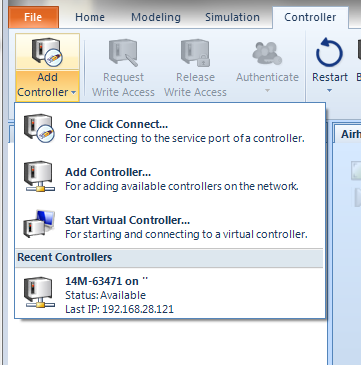
\includegraphics[height=.35\textwidth]{AddController2.png}
\vspace{-15pt}
\caption{Controller hinzufügen} 
\label{controller1}
\end{wrapfigure}

Melden sie sich auf dem Windows-PC mit ihrem DHBW-Account an. Öffnen sie anschließend RobotStudio. Nun müssen sie zunächst unser RobotStudio-Projekt entpacken. Klicken sie dazu in der linken Menüleiste auf \enquote{Share} und dann auf \enquote{Unpack and Work}. Navigieren sie anschließend zum Projektordner und wählen die Datei \enquote{Airhockey2.0.rspag} aus. Legen sie nun einen Speicherort für die das Projekt aus und merken sich diesen, damit es zu einem späteren Zeitpunkt von dort öffnen können. Nach erfolgreichem Entpacken öffnet sich die Station automatisch. 

\begin{wrapfigure}{l}{.4\textwidth}
\centering
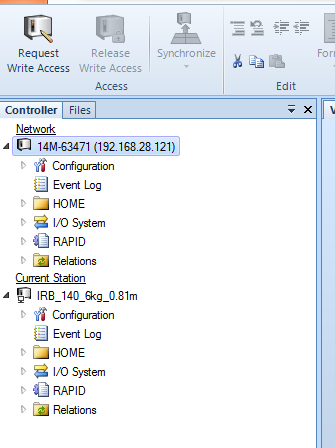
\includegraphics[height=.35\textwidth]{AddController.png}
\vspace{-15pt}
\caption{Verzeichnisstruktur} 
\label{controller2}
\end{wrapfigure}

Als nächstes müssen sie den Roboter einbinden. Stellen sie zunächst sicher, dass er eingeschaltet ist. Gehen sie dann unter den Reiter \enquote{Controller} und dann auf \enquote{Add Controller}. Der Roboter-Controller hat die IP-Adresse 192.168.28.121 und sollte ganz unten im Drop-Down-Menü zu finden sein (siehe Abb. ~\ref{controller1}). Oft muss man um ihn auswählen zu können, das Menü nochmal einklappen und dann erneut auf \enquote{Add Controller} klicken. 

Nach erfolgreichem Einbinden können sie den Roboter in der linken Verzeichnisstruktur finden (vgl. Abb. ~\ref{controller2}). In seinem Unterverzeichnis RAPID finden sie alle Programme, die momentan auf ihm aufgespielt sind. Hier sollten sich nach diesem Schritt die Dateien \enquote{CalibData.mod} und \enquote{positionenAbfahren} befinden. Um diese von \enquote{Current Station} auf den Controller zu übertragen müssen sie eine Verbindung zwischen beiden anlegen. Dies können sie durch die Funktionalität \enquote{Create Relation}, welche sie unter der Registerkarte \enquote{Controller} ganz rechts finden.

Achten sie darauf, dass sie bei der Datenübertragung nur die beiden nötigen Dateien \enquote{positionenAbfahren} und \enquote{CalibData.mod} ausgewählt haben und nicht versehentlich System-Module überschreiben (siehe Abb. ~\ref{transfer}). Bevor sie die Dateien kopieren können, müssen sie Schreibzugriff auf den Controller anfordern. Im Automatik-Modus können sie dies direkt über RobotStudio erlauben. Ist er auf Handbetrieb eingestellt müssen sie dies zunächst auf dem FlexPendant bestätigen.

\begin{figure}[htbp]
\centering
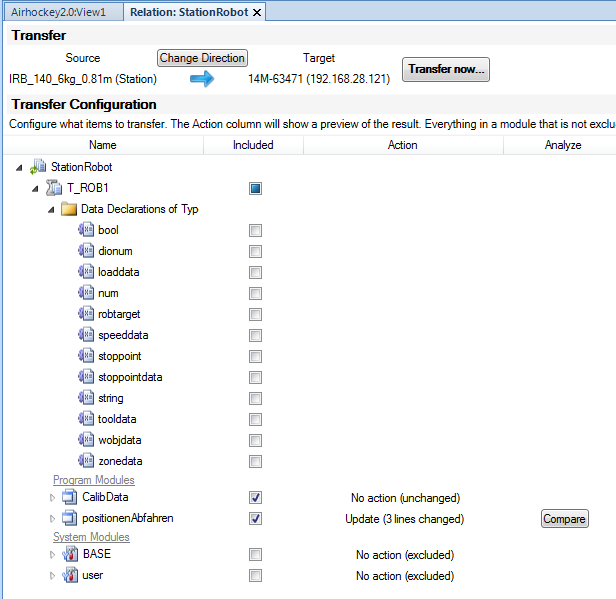
\includegraphics[width=10cm]{transferData2.png}
\caption{Datentransfer auf den Roboter-Controller} 
\label{transfer}
\end{figure}
   

\section{Kalibrierung des Roboters}
Wurde der Roboter längere Zeit nicht mehr benutzt, sollte vor der Benutzung getestet werden, ob der Roboter noch richtig kalibriert ist. Zu diesem Zweck gibt es die Routine \enquote{Kalibrierungstest}. Wird diese ausgeführt, werden mit langsamer Geschwindigkeit die vier Eckpunkte des Bereiches abgefahren in dem er sich bewegen kann, wobei sich Schlägerunterkante 30 mm über der Tischplatte befindet (siehe Listing ~\ref{kali}). Dabei sollte zum einen überprüft werden, ob die Schlägerunterkante überall 3 cm über dem Tisch ist. Dazu das Programm stoppen und an verschiedenen Stellen nachmessen. Außerdem sollte der Schläger genau in die beiden Ecken des Spielfeldes fahren und sich parallel zu den Banden bewegen. Sollte dies nicht der Fall sein, oder man möchte gar einen anderen Schläger verwenden, muss eine Neukalibrierung vorgenommen werden. Dazu müssen die folgenden drei Schritte durchgeführt werden.

\begin{lstlisting}[caption=RAPID-Routine: Kalibrierungstest, label=kali]
!Definitionen der Targets aus der Datei CalibData

CONST robtarget Target_10:=[[xMin,yMin,30],[0,1,0,0],[-1,0,0,0],[9E9,9E9,9E9,9E9,9E9,9E9]];
CONST robtarget Target_20:=[[xMin,yMax,30],[0,1,0,0],[-1,0,0,0],[9E9,9E9,9E9,9E9,9E9,9E9]]; 
CONST robtarget Target_30:=[[xMax,yMax,30],[0,1,0,0],[-1,0,0,0],[9E9,9E9,9E9,9E9,9E9,9E9]];
CONST robtarget Target_40:=[[xMax,yMin,30],[0,1,0,0],[-1,0,0,0],[9E9,9E9,9E9,9E9,9E9,9E9]]; 

! Die Routine Kalibrierungstest aus der Datei positionenAbfahren

PROC Kalibrierungstest()
	MoveL Target_10,v50,fine,tool0\WObj:=Workobject_Table;
   	MoveL Target_20,v50,fine,tool0\WObj:=Workobject_Table;
    MoveL Target_30,v50,fine,tool0\WObj:=Workobject_Table; 
    MoveL Target_40,v50,fine,tool0\WObj:=Workobject_Table; 
        
ENDPROC
\end{lstlisting}

\subsection{Schläger montieren}
Wurde der Schläger demontiert oder möchte man einen neuen Schläger montieren, so muss man den Roboterarm zunächst auf die vordefinierte Home-Position fahren. In dieser Position kann man den Schläger bequem ab- und anschrauben. Viel wichtiger ist jedoch, dass an dieser Position die Orientierung des Werkzeughalters (als Quaternion ausgedrückt) und die Achsenkonfiguration genau die gleichen sind wie bei den Positionsangaben, die dem Roboter später übergeben werden. Man kann den Roboter auf unterschiedliche Arten auf diese Position bringen. Zum einen durch ausführen der Routine \enquote{Jump-Home} in RobotStudio (Automatik-Modus) oder über das FlexPendant (Handbetrieb) (siehe Listing ~\ref{home}). Über das FlexPendant kann die Position (\enquote{Target\_Home}) auch direkt angefahren werden, wobei man dabei darauf achten muss, dass als Koordinatensystem \enquote{Welt}, als Werkzeug \enquote{tool0} und als Workobjekt \enquote{wobj0} eingestellt ist. Bei der Montage des Schlägers muss man anschließend darauf achten, dass der Schläger möglichst parallel zur Roboterachse nach vorne zeigt. 

\begin{lstlisting}[caption=RAPID-Routine: Jump-Home, label=home]
!Definitionen der Home-Position aus der Datei CalibData
CONST robtarget Target_Home:=[[453,26,610],[0,1,0,0],[-1,0,0,0],[9E9,9E9,9E9,9E9,9E9,9E9]];

! Die Routine Jump_Home aus der Datei positionenAbfahren

PROC Jump_Home()
    MoveL Target_Home,v50,fine,tool0\WObj:=wobj0;
ENDPROC
\end{lstlisting} 

\subsection{Eckpunkte abfahren}

Bei diesem Schritt muss man zunächst auf dem FlexPendant als Koordinatensystem \enquote{Welt}, als Werkzeug \enquote{tool0} und als Workobjekt \enquote{wobj0} eingestellen. Danach könne wie in Abbildung ~\ref{eckpunkte} dargestellt, die drei Positionen abgefahren und jeweils die X-,Y- und Z-Koordinaten notiert werden. Dabei darf der Roboter nur lineare bewegt werden. Dabei sollte man bei \enquote{Position 1} möglichst genau in die Ecke fahren, da dies der Ursprung des Werkobjekt-Koordinatensystems ist. 

\begin{figure}[htbp]
\centering
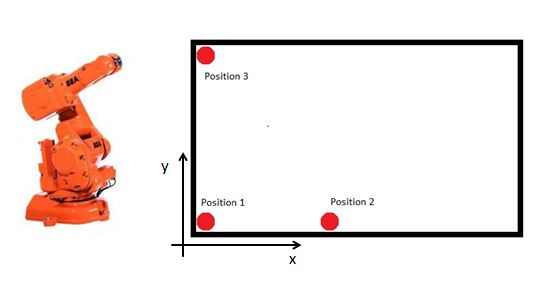
\includegraphics[width=10cm]{Eckpunkte.jpg}
\caption{Die drei Positionen zur Kalibrierung des Roboters} 
\label{eckpunkte}
\end{figure}

\subsection{Workobjekt erzeugen}

\begin{wrapfigure}{l}{.4\textwidth}
\centering
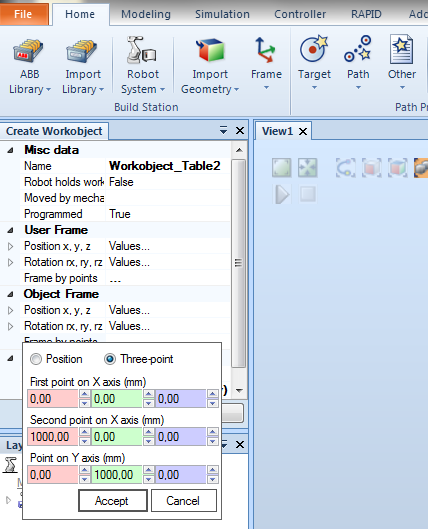
\includegraphics[height=.45\textwidth]{Wobj_anlegen.PNG}
\vspace{-15pt}
\caption{Workobjekt über drei Punkte definieren} 
\label{dreipunkte}
\end{wrapfigure}

Mit Hilfe der notierten Koordinaten, kann in Robotstudio ein neues Workobjekt angelegt werden. Dazu muss auch hier zunächst sichergestellt werden, dass als Koordinatensystem \enquote{Welt}, als Werkzeug \enquote{tool0} und als Workobjekt \enquote{wobj0} eingestellt ist. Zum erzeugen eines neuen Workobjekts klickt man unter dem Reiter \enquote{Home} auf \enquote{Other} und anschließend auf \enquote{Creat Workobjekt}. In der linken Leiste öffnet sich ein entsprechendes Konfigurationmenü. Hier muss man nun das Feld \enquote{Frame by points} ausklappen und den Radio-Button \enquote{Three-point} auswählen (siehe Abb. ~\ref{dreipunkte}). Nun können hier für die drei Punkte die notierten Koordinaten  in der vorgegebenen Reihenfolge eingegeben werden.  

Die Definition diese Workobjekts findet man anschließend in der Datei \enquote{CalibData} der \enquote{Current-Station} im Verzeichnis \enquote{RAPID}. Um diese Datei zu aktualisieren, muss man zunächst eine Synchronisation mit der Station vornehmen. Dafür einfach im Reiter \enquote{RAPID} in der oberen Menüleiste auf \enquote{Sychronize} und dann auf \enquote{Synchronize to RAPID} klicken. 
Übertragen sie anschließend die neuen Daten auf den Roboter. Dies können sie wieder über die \enquote{Relation} machen, oder wenn der Roboter sich im Automatik-Modus befindet auch durch Editieren der Datei \enquote{CalibData} auf dem Controller des Roboters. 
Ersetzen sie dazu die alte Definition von \enquote{wobj\_Table} durch die soeben erstellte. 

\section{Ein Spiel starten}
\label{starten}
In diesem Abschnitt wird Schritt für Schritt beschrieben, wie man ein Spiel startet, wenn an den beiden Rechnern und dem Roboter seit Beendigung unserer Studienarbeit nichts mehr verändert wurde, oder bereits die Anweisungen der beiden vorhergehenden Abschnitte erfolgreich umgesetzt wurden.

\subsection{Roboter-Programm starten} 
Zuerst muss das RAPID-Programm auf dem Roboter-Controller gestartet werden. Dazu müssen folgende sechs Schritte durchgeführt werden:  
\begin{enumerate}
\item Öffnen sie RobotStudio auf dem Windows-PC und öffnen sie die Datei \enquote{Airhockey2.0.rssln}. Sofern sie noch den selben Rechner verwenden finden Sie diese Datei auf Laufwerk C im Ordner \enquote{Airhockey2.0}. Andernfalls in dem Verzeichnis, indem Sie das Projekt entpackt haben. 

\item Stellen sie zunächst sicher, dass er eingeschaltet ist und auf Automatik-Betrieb eingestellt ist. Gehen sie dann in RobotStudio unter dem Reiter \enquote{Controller} auf \enquote{Add Controller}. Der Roboter-Controller hat die IP-Adresse 192.168.28.121 und sollte ganz unten im Drop-Down-Menü zu finden sein (siehe Abb. ~\ref{controller1}). Oft muss man um ihn auswählen zu können, das Menü nochmal einklappen und dann erneut auf \enquote{Add Controller} klicken.

\item Wechseln sie in den Reiter \enquote{RAPID} und öffnen sie die Datei \enquote{positioinenAbfahren} im Verzeichnis \enquote{RAPID} aus dem Roboter-Controller (14M-63471(192.168.28.121))(siehe Abb. ~\ref{controller2}). Fordern sie nun Schreibzugriff auf den Roboter-Controller an, indem sie auf den Knopf \enquote{Request Write Acces} drücken. 

\item Starten sie die Motoren des Roboters durch drücken von Schalter 3 am Schaltschrank(siehe Abb. ~\ref{schaltschrank}).

\item Setzen sie als nächstes den Programm-Zeiger zurück. Klicken sie dazu auf \enquote{Program Pointer} und wählen sie dann \enquote{Set Program Pointer to Main in all tasks}. Diesen Schritt müssen auch vor jedem weiteren Start des Programmes durchführen, da zu Beginn immer erst eine Verbindung mit der Bilderkennung aufgebaut werden muss.

\item Als letztes betätigen sie in RobotStudio den Start-Knopf. Der Schläger wird dann sofort in die Mitte des Tores gefahren, bevor versucht wird eine Verbindung mit der Bilderkennung aufzubauen.    
\end{enumerate}

\subsection{Bildverarbeitung starten}
\begin{enumerate}
\item Stellen sie zunächst sicher, dass die Kamera an den Linux-Rechner angeschlossen ist.

\item Öffnen sie das Terminal und navigieren sie ins Verzeichnis \enquote{Schreibtisch/Airhockey/airhockey}


\begin{figure}[htbp]
\centering
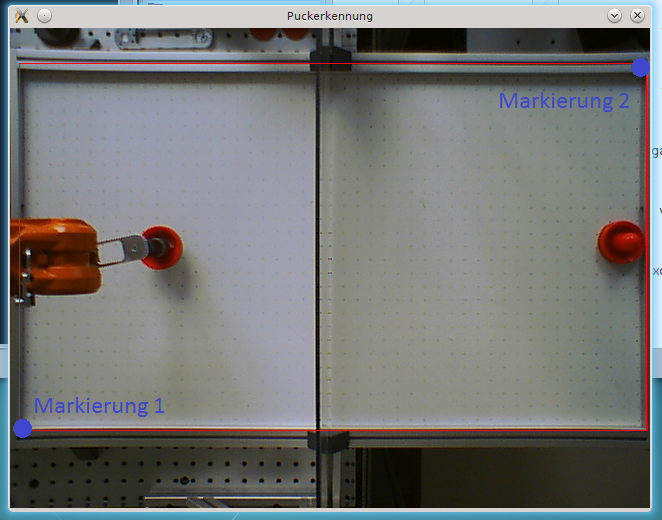
\includegraphics[width=12cm]{spielfeld.png}
\caption{Einzeichnen des Spielfeldes} 
\label{spielfeld}
\end{figure}

\item Starten sie die Bilderkennung, indem sie hier das Skript \enquote{table\_setup.sh} ausführen. Dieses erwartet zwei Interger-Werte als Übergabeparameter. Zum einen den Kameraanschluss und zum anderen die Framerate, mit der die Kamera aufnehmen soll. Den Kameraanschluss findet man im Verzeichnis \enquote{/dev} heraus. Suchen sie hier nach Ordnern, die mit \enquote{video} beginnen. Ist nur eine Kamera angeschlossen, sollte ein Ordner \enquote{video0} existieren. Der erste Übergabewert wäre somit 0. Als Framerrate sollten 30 Bilder pro Sekunde genutzt werden. Der Befehl zum Starten des Skripts ergibt sich damit wie folgt:

\begin{lstlisting}[caption=Terminal-Befahl zum starten der Bilderkennung, label=start, language=bash]
sh table_setup 0 30
\end{lstlisting} 

\item Das Programm versucht nun zunächst eine Verbindung mit dem Roboter-Controller auf zu bauen. Erst wenn dies erfolgreich war, öffnet sich ein Fenster, in dem ein Standbild des Tisches zu sehen ist. Darin muss nun zunächst das Spielfeld eingezeichnet werden. Dazu müssen sie zunächst den die untere linke Ecke und anschließend die obere rechte Ecke des Spielfeldes mit einem Doppelklick markieren (siehe Abb. ~\ref{spielfeld}). Dabei ist sehr wichtig, dass die Punkte genau in dieser Reihenfolge markiert werden, da ansonsten die Bilderkennung ein falsches Koordinatensystem zur Berechnung verwendet.   

\item Haben sie alle vorherigen Schritte erfolgreich abgearbeitet, können sie nun Air-Hockey gegen den Roboter spielen. Wir wünschen ihnen viel Spaß dabei. Zum Beenden des Bilderkennung einfach in im Terminal \enquote{Strg + C} eingeben.   

\end{enumerate} 

